% Options for packages loaded elsewhere
\PassOptionsToPackage{unicode}{hyperref}
\PassOptionsToPackage{hyphens}{url}
%
\documentclass[
]{article}
\usepackage{amsmath,amssymb}
\usepackage{lmodern}
\usepackage{iftex}
\ifPDFTeX
  \usepackage[T1]{fontenc}
  \usepackage[utf8]{inputenc}
  \usepackage{textcomp} % provide euro and other symbols
\else % if luatex or xetex
  \usepackage{unicode-math}
  \defaultfontfeatures{Scale=MatchLowercase}
  \defaultfontfeatures[\rmfamily]{Ligatures=TeX,Scale=1}
\fi
% Use upquote if available, for straight quotes in verbatim environments
\IfFileExists{upquote.sty}{\usepackage{upquote}}{}
\IfFileExists{microtype.sty}{% use microtype if available
  \usepackage[]{microtype}
  \UseMicrotypeSet[protrusion]{basicmath} % disable protrusion for tt fonts
}{}
\makeatletter
\@ifundefined{KOMAClassName}{% if non-KOMA class
  \IfFileExists{parskip.sty}{%
    \usepackage{parskip}
  }{% else
    \setlength{\parindent}{0pt}
    \setlength{\parskip}{6pt plus 2pt minus 1pt}}
}{% if KOMA class
  \KOMAoptions{parskip=half}}
\makeatother
\usepackage{xcolor}
\usepackage[margin=1in]{geometry}
\usepackage{longtable,booktabs,array}
\usepackage{calc} % for calculating minipage widths
% Correct order of tables after \paragraph or \subparagraph
\usepackage{etoolbox}
\makeatletter
\patchcmd\longtable{\par}{\if@noskipsec\mbox{}\fi\par}{}{}
\makeatother
% Allow footnotes in longtable head/foot
\IfFileExists{footnotehyper.sty}{\usepackage{footnotehyper}}{\usepackage{footnote}}
\makesavenoteenv{longtable}
\usepackage{graphicx}
\makeatletter
\def\maxwidth{\ifdim\Gin@nat@width>\linewidth\linewidth\else\Gin@nat@width\fi}
\def\maxheight{\ifdim\Gin@nat@height>\textheight\textheight\else\Gin@nat@height\fi}
\makeatother
% Scale images if necessary, so that they will not overflow the page
% margins by default, and it is still possible to overwrite the defaults
% using explicit options in \includegraphics[width, height, ...]{}
\setkeys{Gin}{width=\maxwidth,height=\maxheight,keepaspectratio}
% Set default figure placement to htbp
\makeatletter
\def\fps@figure{htbp}
\makeatother
\setlength{\emergencystretch}{3em} % prevent overfull lines
\providecommand{\tightlist}{%
  \setlength{\itemsep}{0pt}\setlength{\parskip}{0pt}}
\setcounter{secnumdepth}{5}
\newlength{\cslhangindent}
\setlength{\cslhangindent}{1.5em}
\newlength{\csllabelwidth}
\setlength{\csllabelwidth}{3em}
\newlength{\cslentryspacingunit} % times entry-spacing
\setlength{\cslentryspacingunit}{\parskip}
\newenvironment{CSLReferences}[2] % #1 hanging-ident, #2 entry spacing
 {% don't indent paragraphs
  \setlength{\parindent}{0pt}
  % turn on hanging indent if param 1 is 1
  \ifodd #1
  \let\oldpar\par
  \def\par{\hangindent=\cslhangindent\oldpar}
  \fi
  % set entry spacing
  \setlength{\parskip}{#2\cslentryspacingunit}
 }%
 {}
\usepackage{calc}
\newcommand{\CSLBlock}[1]{#1\hfill\break}
\newcommand{\CSLLeftMargin}[1]{\parbox[t]{\csllabelwidth}{#1}}
\newcommand{\CSLRightInline}[1]{\parbox[t]{\linewidth - \csllabelwidth}{#1}\break}
\newcommand{\CSLIndent}[1]{\hspace{\cslhangindent}#1}
\usepackage{float}
\floatplacement{figure}{H}
\usepackage{booktabs}
\usepackage{longtable}
\usepackage{array}
\usepackage{multirow}
\usepackage{wrapfig}
\usepackage{float}
\usepackage{colortbl}
\usepackage{pdflscape}
\usepackage{tabu}
\usepackage{threeparttable}
\usepackage{threeparttablex}
\usepackage[normalem]{ulem}
\usepackage{makecell}
\usepackage{xcolor}
\ifLuaTeX
  \usepackage{selnolig}  % disable illegal ligatures
\fi
\IfFileExists{bookmark.sty}{\usepackage{bookmark}}{\usepackage{hyperref}}
\IfFileExists{xurl.sty}{\usepackage{xurl}}{} % add URL line breaks if available
\urlstyle{same} % disable monospaced font for URLs
\hypersetup{
  pdftitle={Analysis of Physical Activity Survey(2022)},
  pdfauthor={Jonathan Goodwin},
  hidelinks,
  pdfcreator={LaTeX via pandoc}}

\title{Analysis of Physical Activity Survey(2022)}
\author{Jonathan Goodwin}
\date{12 February 2023}

\begin{document}
\maketitle
\begin{abstract}
Recreational activity and physical fitness are important factors in determining the health and safety of a society. We obtain data regarding the activity of individuals of different states and age groups as well as their respective distance to a park. We find that citizens who live closer to parks are more likely to be physically active, and that younger citizens are more likely to be physically active then older ones. These findings have implications for the future development of public recreational structures.
\end{abstract}

\hypertarget{keywords}{%
\section{Keywords:}\label{keywords}}

Health, Physical Activity, Recreation, United States, Survey

\hypertarget{Intro}{%
\section{Introduction}\label{Intro}}

Physical activity is an important indicator for the health of the population of the United States. As well living near to a public recreational service like a park allows residents a more convenient place to excercise. We see that decreasing the distance to a park as well as giving more opportunity for residents to participate in activities like biking is associated with more physically active residents who meet the CDC's guidelines for strength and aerobic health.

We analyzed the sources of water for two subsets of the Jordan population, urban and rural residents. From Table \ref{tab:tab2} and Table \ref{tab:tab3}, we can see that both Colorado is the state with the lowest rate of obesity and that Mississipi is the highest.

This information is relevant to the further development and enhancement of the recreational and physical activity of citizens of the United States as well as leader of respective states when developing cities. The data can help to identify populaces with particularly low activity reletive to the rest of the country as well as identify states that are lacking in public recreational support for its citizens.

Overall we found that the state with the highest rates of Obesity was Mississipi, the lowest was Colorado and that there is a relationship between the proportion of state residents participating in recreational activities like muscle training or aerobics and the obesity rate of residents within that state.

In section \ref{Data} we talk about the process of gathering and analyzing the dataset and the variables. Then in section \ref{Model} we build a linear model for the rate of obesity. Then in section \ref{Results} we discuss the implications of the dataset presented. Finally in section \ref{Discussion} we discuss implications for the United States citizens, as well as the weakness of the study and the further investigation that may be useful to the topic of recreational activity support and physical activity in the United States.

\newpage

\hypertarget{Data}{%
\section{Data}\label{Data}}

The dataset is from the National Health Interview Survey. The survey was conducted by the Centers for Disease Control and Prevention, (\emph{Nutrition, Physical Activity, and Obesity} 2022) and the data used was from the years 2010 to 2020.The survey was conducted and funded by the CDC but also has numerous sponsors found \href{https://www.cdc.gov/nchs/nhis/supplements_cosponsors.htm}{here}.

The survey has been conducted every year for over 50 years, the sample is nationally representative, the intent of the survey is to monitor the health of the nation, as it collects information by interviewing American households. The content of the survey is updated roughly every 15-20 years with the most recent being in 2019. Of which 30,000 adults and 9,000 children were interviewed. Of this survey, this analysis focused on the information regarding the proportion of adults classified as obese or overweight, and how they responded to questions regarding aerobic activity and weight training. The data is collected from all 50 states including the District of Columbia, there is also a section included for the National averages of each question response.

To compile the data set, the R language was used(R Core Team 2020), along with the packages, Pointblank (Iannone and Vargas 2022), haven (Wickham and Miller 2021), the paper was compiled using Knitr (Xie 2021) and KableExtra(Zhu 2021) packages. Also made use of reshape2 (Wickham 2007) in manipulating the data to create plots.

Table \ref{tab:tab1} gives a small look at the dataset.

\begin{table}[!h]

\caption{\label{tab:tab1}Excerpt of dataset}
\centering
\begin{tabular}[t]{ccccc}
\toprule
Year & State & Question & Percent & Age\\
\midrule
2011 & Alabama & Percent of adults aged 18 years and older who have obesity & 35.2 & 25 - 34\\
2011 & National & Percent of adults who engage in no leisure-time physical activity & 16.9 & 18 - 24\\
2016 & Virginia & Percent of adults aged 18 years and older who have an overweight classification & 40.1 & 35 - 44\\
2016 & Washington & Percent of adults who engage in no leisure-time physical activity & 18.8 & 55 - 64\\
2016 & Alabama & Percent of adults aged 18 years and older who have an overweight classification & 35.3 & 55 - 64\\
\addlinespace
2011 & National & Percent of adults who engage in no leisure-time physical activity & 22.1 & 25 - 34\\
\bottomrule
\end{tabular}
\end{table}

In total there are 6 characteristics from the survey being analyzed, they are:

\begin{enumerate}
\def\labelenumi{\arabic{enumi}.}
\item
  ``Percent of adults aged 18 years and older who have obesity''\\
\item
  ``Percent of adults aged 18 years and older who have an overweight classification''\\
\item
  ``Percent of adults who engage in no leisure-time physical activity''\\
\item
  ``Percent of adults who achieve at least 150 minutes a week of moderate-intensity aerobic physical activity or 75 minutes a week of vigorous-intensity aerobic activity (or an equivalent combination)''
\item
  ``Percent of adults who engage in muscle-strengthening activities on 2 or more days a week''\\
\item
  ``Percent of adults who achieve at least 300 minutes a week of moderate-intensity aerobic physical activity or 150 minutes a week of vigorous-intensity aerobic activity (or an equivalent combination)''
\end{enumerate}

These are stratified into 6 different age groups for adults, those 18-24, 25-34, 35-44, 45-54, 55-64, and 65 and older.

The responses are given as a proportion of the sample, rounded to 1 digit. So the value 35.2 means, 35.2\% of respondents in that age group had been affirmative to that trait in the survey.

\newpage

\hypertarget{Model}{%
\section{Model}\label{Model}}

The model being used is \(\text{Obesity}=\beta_{\text{Intercept}}+\beta_{\text{150min of Aerobics}}\times (\text{150min of Aerobics or more})+\beta_{\text{Muscle Training}}\times (\text{Muscle Training})\). Where the beta coefficients represent the change in the predictor variables, 150min or more of Aerobics, and Muscle Training, have on the result, being the obesity rate. This model was chosen since other factors like no aerobic activity or 300min or more of aerobic activity were unsuprisingly highly correlated with the 150min of aerobics.

Both Muscle Training and 150min of Aerobic Training had significant p-values in this model of 0.0236 and 0.0027 respectively. Below Figure \ref{fig:fig5} shows the relationship between 150min of Aerobics training and Muscle Training compared to the rate of Obesity. There was strong positive correlation to people with 300min of aerobic training, and those who did muscle training or 150min of aerobic training so including that interaction was not beneficial. Additionally those that do no aerobic training at all are strongly negatively correlated with those that do 150min or more. Soi including that interaction was not beneficial to the model.

Our data does not have any particularly large outliers that would disturb the model present. And our outcome variable, the proportion of residents who are obese is a continuous variable, thus the bilinear model seems the best choice.

\begin{figure}
\centering
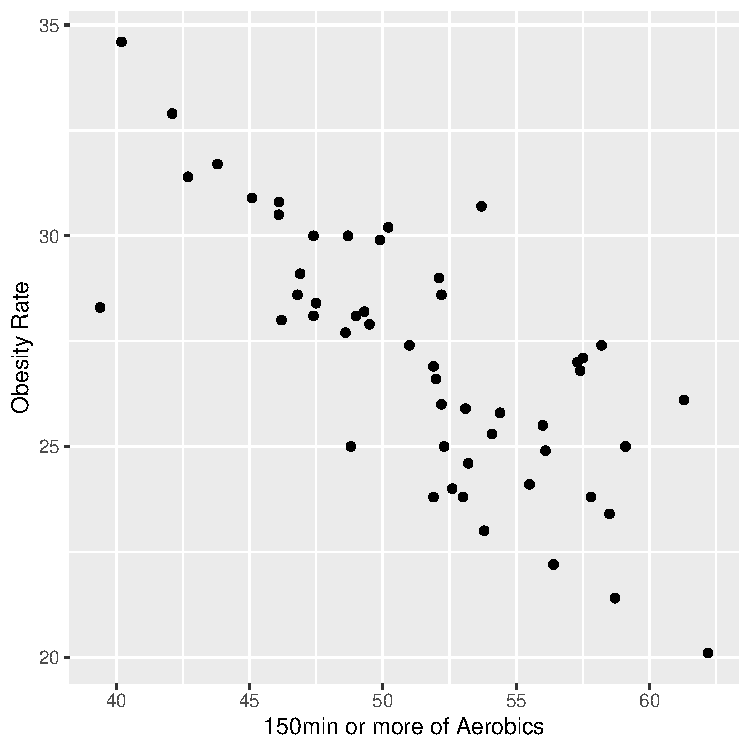
\includegraphics{paper_files/figure-latex/fig5-1.pdf}
\caption{\label{fig:fig5}Obesity vs 150min of Aerobics}
\end{figure}

And below Figure \ref{fig:fig6} shows us the relationship between the rate of obesity and the proportion of a states residents participating in muscle training excercises.

\begin{figure}
\centering
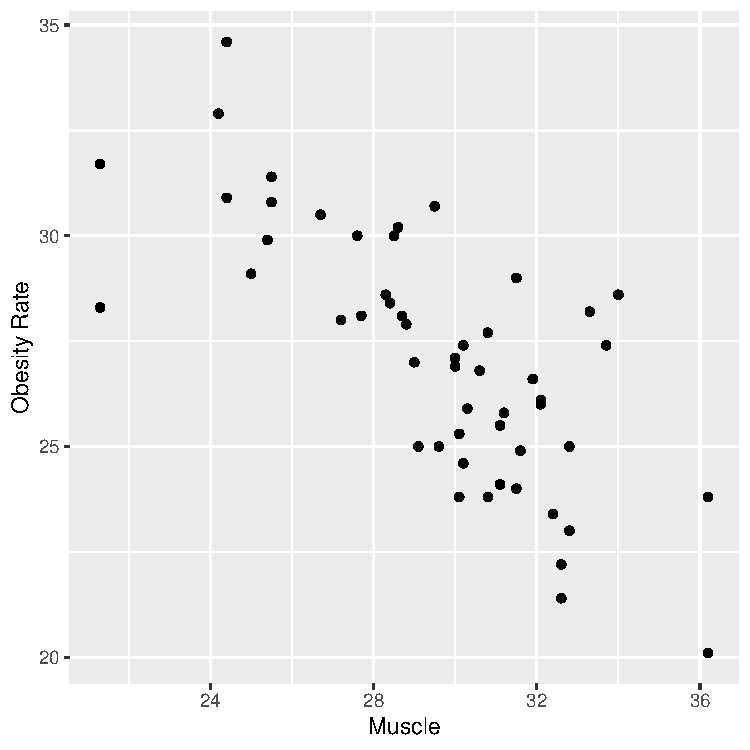
\includegraphics{paper_files/figure-latex/fig6-1.pdf}
\caption{\label{fig:fig6}Obesity vs Muscle Training}
\end{figure}

\newpage

\hypertarget{Results}{%
\section{Results}\label{Results}}

From Figure \ref{fig:fig1} we see a chart comparing the proportion of respondents who were obese based on the different states in the country. We can see from the chart that all states lie between a rate of 20\% and 35\% obese. The chart below is for 2011.

\begin{figure}
\centering
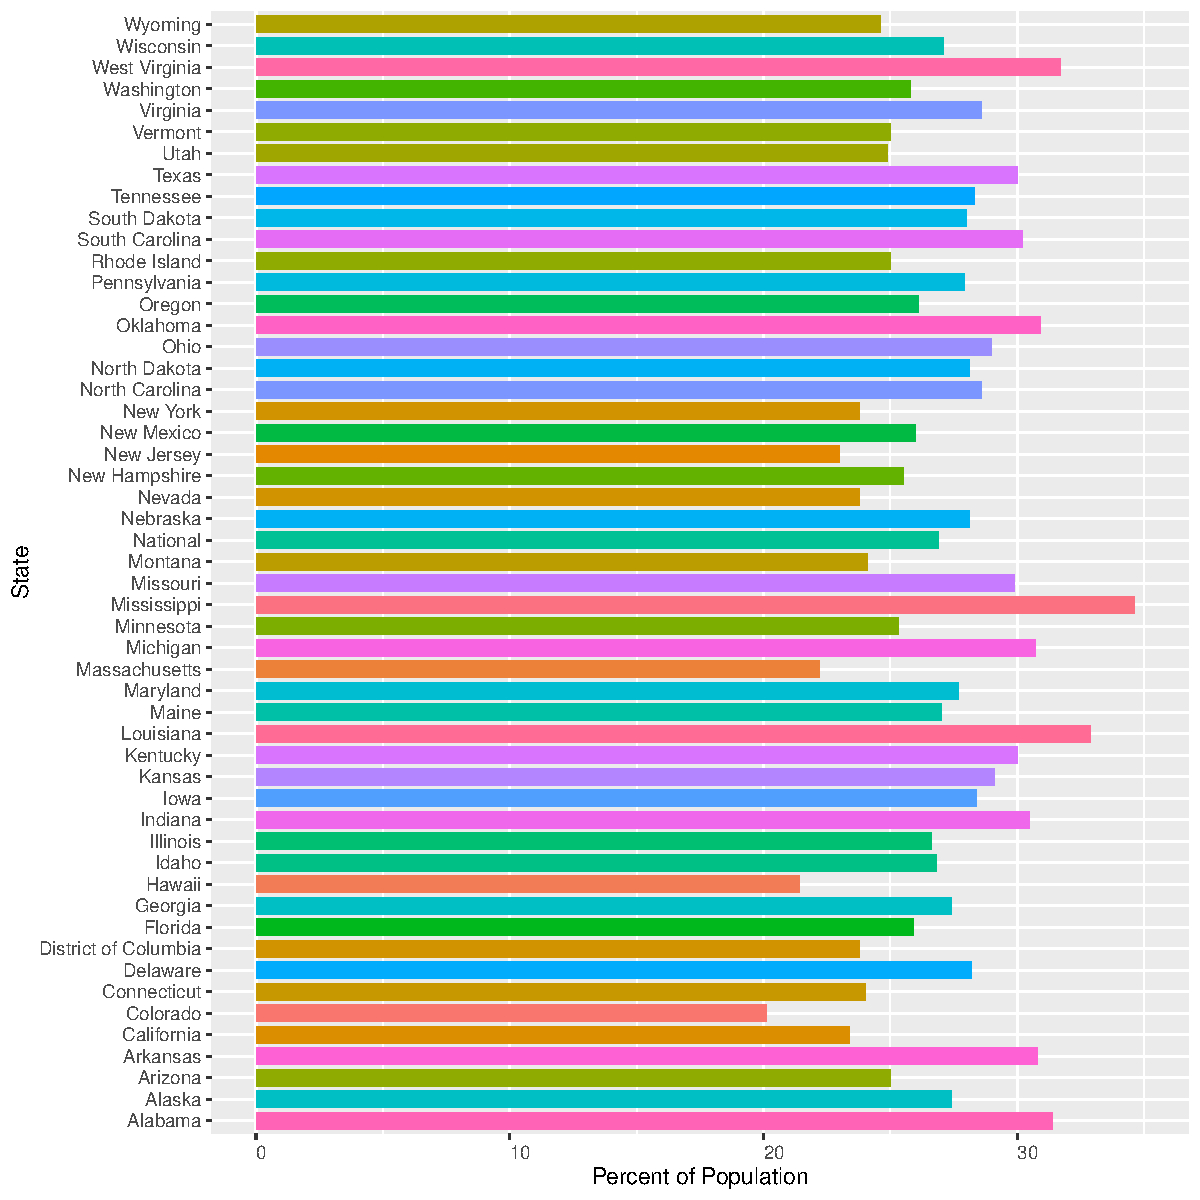
\includegraphics{paper_files/figure-latex/fig1-1.pdf}
\caption{\label{fig:fig1}Bar plot of Obesity by State}
\end{figure}

Below Table \ref{tab:tab2}, shows the states with the lowest proportions of obesity.

\begin{table}[H]

\caption{\label{tab:tab2}Lowest Obesity Rates By State}
\centering
\begin{tabular}[t]{cc}
\toprule
Colorado & 20.1\\
Hawaii & 21.4\\
Massachusetts & 22.2\\
New Jersey & 23\\
California & 23.4\\
\addlinespace
District of Columbia & 23.8\\
\bottomrule
\end{tabular}
\end{table}

And here Table \ref{tab:tab3} gives the states with the highest obesity rates.

\begin{table}[H]

\caption{\label{tab:tab3}Highest Obesity Rates by State}
\centering
\begin{tabular}[t]{cc}
\toprule
Mississippi & 34.6\\
Louisiana & 32.9\\
West Virginia & 31.7\\
Alabama & 31.4\\
Oklahoma & 30.9\\
\addlinespace
Arkansas & 30.8\\
\bottomrule
\end{tabular}
\end{table}

From these tables and the chart above we see the lowest obesity rate in the United States is Colorado with 20.1\% and the highest is Mississippi with 34.6\%. For this analysis we want to see whether physical activity factors such as aerobic excercise. Below in \ref{fig:fig2} however we will briefly see how these obesity rates have changed by the end of the decade.

\begin{figure}
\centering
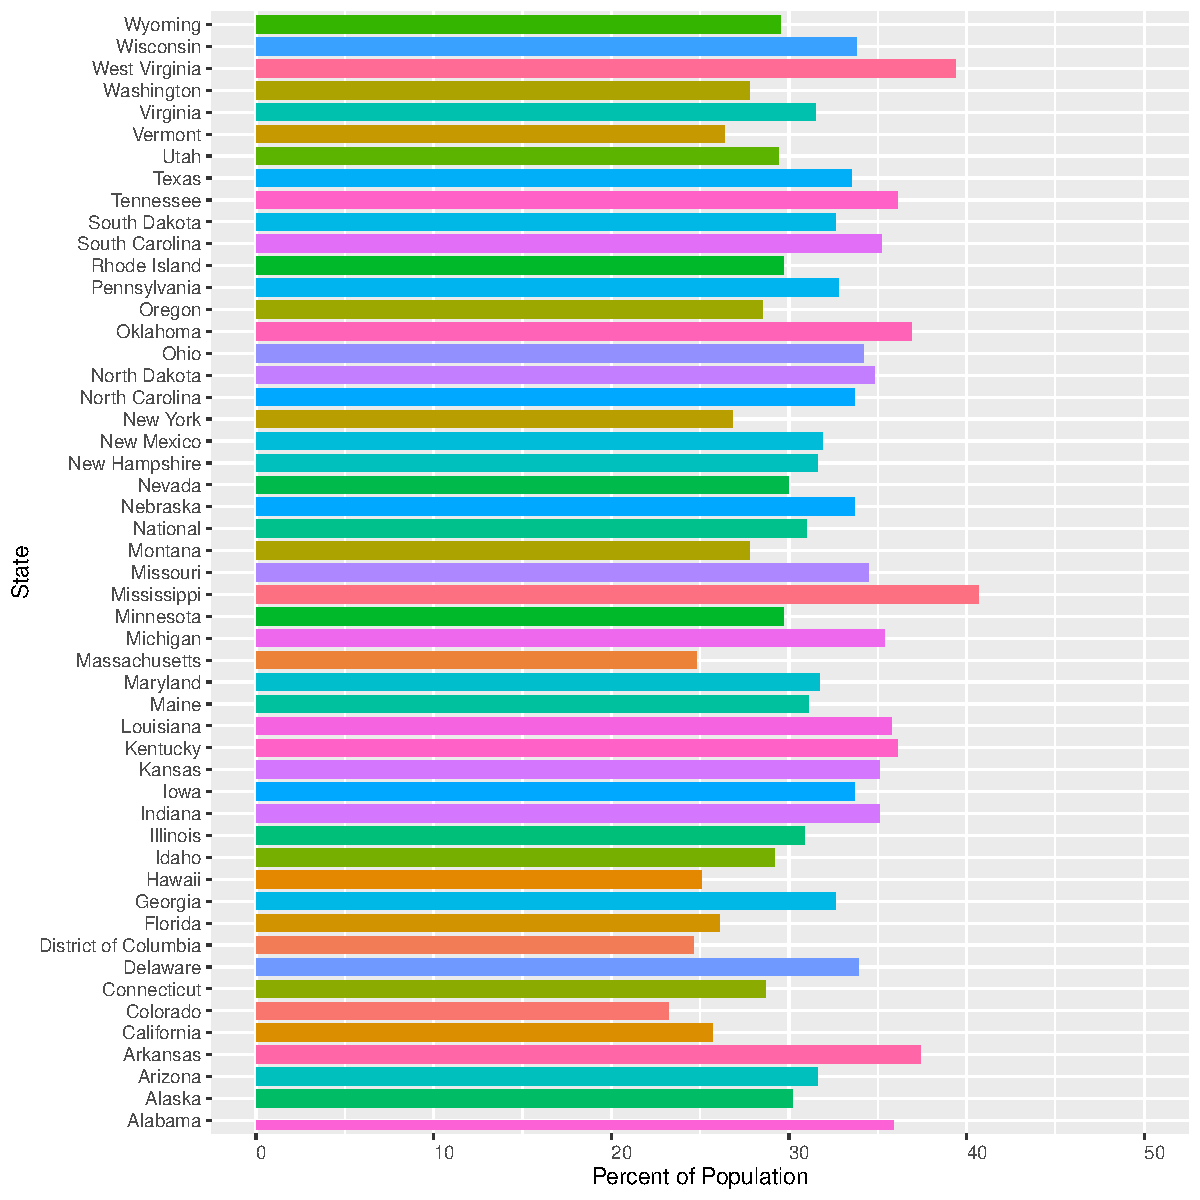
\includegraphics{paper_files/figure-latex/fig2-1.pdf}
\caption{\label{fig:fig2}Bar plot of Obesity by State}
\end{figure}

We see from \ref{fig:fig2} that the overall rate of obesity has clearly increased, however the states with the highest and lowest rates remain largely the same as we can see from Table \ref{tab:tab4} and Table \ref{tab:tab5} below.

\begin{table}[H]

\caption{\label{tab:tab4}Lowest Rates of Obesity by State}
\centering
\begin{tabular}[t]{cc}
\toprule
Colorado & 23.2\\
District of Columbia & 24.6\\
Massachusetts & 24.8\\
Hawaii & 25.1\\
California & 25.7\\
\addlinespace
Florida & 26.1\\
\bottomrule
\end{tabular}
\end{table}

\begin{table}[H]

\caption{\label{tab:tab5}Highest Rates of Obesity by State}
\centering
\begin{tabular}[t]{cc}
\toprule
Mississippi & 40.7\\
West Virginia & 39.4\\
Arkansas & 37.4\\
Oklahoma & 36.9\\
Kentucky & 36.1\\
\addlinespace
Tennessee & 36.1\\
\bottomrule
\end{tabular}
\end{table}

Below we now look at the proportion of state residents participating in aerobic activities for 150min or more per week as well as the proportion of residents participating in muscle strength training for at least 2 hours per week. We see in Table \ref{tab:tab10} and Table \ref{tab:tab11} some familiar states from the Obesity rate Tables \ref{tab:tab4} and Table \ref{tab:tab5}. Namely Alabama which was one of the highest rates for Obesity in the country also has low rates of Aerobic activity.

\begin{table}[H]

\caption{\label{tab:tab10}States with Lowest rates of Aerobic training}
\centering
\begin{tabular}[t]{cc}
\toprule
Kentucky & 36.9\\
Oklahoma & 38.1\\
Mississippi & 39.7\\
Missouri & 45.1\\
Louisiana & 45.9\\
\addlinespace
Alabama & 46.1\\
\bottomrule
\end{tabular}
\end{table}

\begin{table}[H]

\caption{\label{tab:tab11}States with Highest rates of Aerobic training}
\centering
\begin{tabular}[t]{cc}
\toprule
Montana & 63\\
Vermont & 61.8\\
Colorado & 59.3\\
Washington & 58.7\\
Minnesota & 58.1\\
\addlinespace
Alaska & 57.5\\
\bottomrule
\end{tabular}
\end{table}

We now look at muscle training in Tables \ref{tab:tab12} and Table \ref{tab:tab13}. Here we see many of the low obesity rate states from earlier, like Colorado, Florida and the District of Columbia.

\begin{table}[H]

\caption{\label{tab:tab12}States with Lowest rates of Muscle Training}
\centering
\begin{tabular}[t]{cc}
\toprule
West Virginia & 27.5\\
Kentucky & 28.1\\
Missouri & 28.7\\
Oklahoma & 29.2\\
Mississippi & 29.8\\
\addlinespace
Alabama & 30\\
\bottomrule
\end{tabular}
\end{table}

\begin{table}[H]

\caption{\label{tab:tab13}States with Highest rates of Muscle training}
\centering
\begin{tabular}[t]{cc}
\toprule
Montana & 40.3\\
District of Columbia & 40.2\\
Connecticut & 39.8\\
Vermont & 39.7\\
Colorado & 39.6\\
\addlinespace
Florida & 38.8\\
\bottomrule
\end{tabular}
\end{table}

The interesting thing here is we see Montana and Vermont both with very high rates of Aerobic Activity, likely attributed to these states being far more rural then the average state, allowing more opportunity for outdoor activities. However again on the low end
\newpage

\hypertarget{Discussion}{%
\section{Discussion}\label{Discussion}}

\hypertarget{FirstPoint}{%
\subsection{FirstPoint}\label{FirstPoint}}

According to (Jason A Bennie 1, n.d.) ``meeting both aerobic and muscle-strengthening exercise guidelines was associated with a lower obesity prevalence, and associations were more pronounced for higher obesity classes.'' We found similar section \ref{Results}. However we also noted in the model that muscle training and aerobic activities did not fully explain the obesity problems of the United States. Suggesting that while physical activity may be important it is not the entire explanation for the increasing rates of obesity. Research suggest Americans currently consume too many calories, saturated fats, trans fasts and added sugars.((US) 2010).

The CDC notes that the solution to obesity in the United States is not simple (Disease Control and Prevention 2022). The CDC notes the solutions are a healthy lifestyle, combining physical activity with healthy eating. They provide plans like the MyPlate Plan to help United States citizens plan their meals and exercise to ensure they are meeting health recommendations.

Some State's have implemented more directly punitive measures to curb obesity, Sugar tax and other so called `sin taxes' have been implemented in cities such as Philadelphia, Boulder, Colorado, and Berkeley, California (Newman 2019) and according to The American Public Health Association these taxes results in a 21\% drop in consumption of sugary drinks in Berkeley (al. 2016). However in past efforts to cap the availability of junk foods and sodas has been struck down by United States courts. Famously in New York City's ban on large quantity soda's was fought in court and ultimately defeated (Grynbaum 2014), with help in no small part to the soft drink industry spending millions on ad campaigns. Industries built around sugary foods and drinks are large and will fight against measures which may reduce the consumption of their products.

\hypertarget{weaknesses-and-next-steps}{%
\subsection{Weaknesses and next steps}\label{weaknesses-and-next-steps}}

Although this analysis found some links between aerobic activity and muscle training to rates of obesity in the United States. It is clear that there is more to the story of obesity in the United States then just the level of physical activity. Next steps for analysis would be researching diet along with exercise. Data in this area in the last 2 years during the pandemic would also be particularly interesting. Particularly in comparing states which had more restricted access to public fitness facilities like gyms and public parks compared to those states which did not employ as strict restrictions, re-opened earlier, or states like Montana which had less population density and more opportunity to open air fitness training compared to densely populated states such as New York.

\newpage

\appendix

\hypertarget{appendix}{%
\section*{Appendix}\label{appendix}}
\addcontentsline{toc}{section}{Appendix}

\hypertarget{datasheet}{%
\subsection*{DataSheet}\label{datasheet}}
\addcontentsline{toc}{subsection}{DataSheet}

\textbf{Motivation}

\begin{enumerate}
\def\labelenumi{\arabic{enumi}.}
\tightlist
\item
  \emph{For what purpose was the dataset created? Was there a specific task in mind? Was there a specific gap that needed to be filled? Please provide a description.}

  \begin{itemize}
  \tightlist
  \item
    The dataset was created to analyze the responses from National Health Interview Survey regarding physical activity.
  \end{itemize}
\item
  \emph{Who created the dataset (for example, which team, research group) and on behalf of which entity (for example, company, institution, organization)?}

  \begin{itemize}
  \tightlist
  \item
    Jonathan Goodwin
  \end{itemize}
\item
  \emph{Who funded the creation of the dataset? If there is an associated grant, please provide the name of the grantor and the grant name and number.}

  \begin{itemize}
  \tightlist
  \item
    No one.
  \end{itemize}
\item
  \emph{Any other comments?}

  \begin{itemize}
  \tightlist
  \item
    No.
  \end{itemize}
\end{enumerate}

\textbf{Composition}

\begin{enumerate}
\def\labelenumi{\arabic{enumi}.}
\tightlist
\item
  \emph{What do the instances that comprise the dataset represent (for example, documents, photos, people, countries)? Are there multiple types of instances (for example, movies, users, and ratings; people and interactions between them; nodes and edges)? Please provide a description.}

  \begin{itemize}
  \tightlist
  \item
    Each row of the dataset corresponds to a the proportion of intervewees that responded affirmatively to a question by year and stratified by age group.
  \end{itemize}
\item
  \emph{How many instances are there in total (of each type, if appropriate)?}

  \begin{itemize}
  \tightlist
  \item
    There are 6 questions, 6 age categories, over the course of 10 years for all 53 states, resulting in 14,196 different entries.
  \end{itemize}
\item
  \emph{Does the dataset contain all possible instances or is it a sample (not necessarily random) of instances from a larger set? If the dataset is a sample, then what is the larger set? Is the sample representative of the larger set (for example, geographic coverage)? If so, please describe how this representativeness was validated/verified. If it is not representative of the larger set, please describe why not (for example, to cover a more diverse range of instances, because instances were withheld or unavailable).}

  \begin{itemize}
  \tightlist
  \item
    The dataset is a sample from the larger National Health Interview Survey conducted by the CDC.
  \end{itemize}
\item
  \emph{What data does each instance consist of? ``Raw'' data (for example, unprocessed text or images) or features? In either case, please provide a description.}

  \begin{itemize}
  \tightlist
  \item
    Each instance consists of a numeric value for the proportion of respondents which responded affirmatively to that question in the survey.
  \end{itemize}
\item
  \emph{Is there a label or target associated with each instance? If so, please provide a description.}

  \begin{itemize}
  \tightlist
  \item
    No.
  \end{itemize}
\item
  \emph{Is any information missing from individual instances? If so, please provide a description, explaining why this information is missing (for example, because it was unavailable). This does not include intentionally removed information, but might include, for example, redacted text.}

  \begin{itemize}
  \tightlist
  \item
    No.
  \end{itemize}
\item
  \emph{Are relationships between individual instances made explicit (for example, users' movie ratings, social network links)? If so, please describe how these relationships are made explicit.}

  \begin{itemize}
  \tightlist
  \item
    No.
  \end{itemize}
\item
  \emph{Are there recommended data splits (for example, training, development/validation, testing)? If so, please provide a description of these splits, explaining the rationale behind them.}

  \begin{itemize}
  \tightlist
  \item
    No.
  \end{itemize}
\item
  \emph{Are there any errors, sources of noise, or redundancies in the dataset? If so, please provide a description.}

  \begin{itemize}
  \tightlist
  \item
    No.
  \end{itemize}
\item
  \emph{Is the dataset self-contained, or does it link to or otherwise rely on external resources (for example, websites, tweets, other datasets)? If it links to or relies on external resources, a) are there guarantees that they will exist, and remain constant, over time; b) are there official archival versions of the complete dataset (that is, including the external resources as they existed at the time the dataset was created); c) are there any restrictions (for example, licenses, fees) associated with any of the external resources that might apply to a dataset consumer? Please provide descriptions of all external resources and any restrictions associated with them, as well as links or other access points, as appropriate.}

  \begin{itemize}
  \tightlist
  \item
    The dataset does not rely on any external sources.
  \end{itemize}
\item
  \emph{Does the dataset contain data that might be considered confidential (for example, data that is protected by legal privilege or by doctor-patient confidentiality, data that includes the content of individuals' non-public communications)? If so, please provide a description.}

  \begin{itemize}
  \tightlist
  \item
    No, the data is all publicly available from the Department of statistics Jordan and required no special permissions to access.
  \end{itemize}
\item
  \emph{Does the dataset contain data that, if viewed directly, might be offensive, insulting, threatening, or might otherwise cause anxiety? If so, please describe why.}

  \begin{itemize}
  \tightlist
  \item
    No.
  \end{itemize}
\item
  \emph{Does the dataset identify any sub-populations (for example, by age, gender)? If so, please describe how these subpopulations are identified and provide a description of their respective distributions within the dataset.}

  \begin{itemize}
  \tightlist
  \item
    The data is split into 6 age groups, 18-24, 24-35, 35-45, 45-55, 55-64, and 65 and older.
  \end{itemize}
\item
  \emph{Is it possible to identify individuals (that is, one or more natural persons), either directly or indirectly (that is, in combination with other data) from the dataset? If so, please describe how.}

  \begin{itemize}
  \tightlist
  \item
    No individuals can be identified from the dataset.
  \end{itemize}
\item
  \emph{Does the dataset contain data that might be considered sensitive in any way (for example, data that reveals race or ethnic origins, sexual orientations, religious beliefs, political opinions or union memberships, or locations; financial or health data; biometric or genetic data; forms of government identification, such as social security numbers; criminal history)? If so, please provide a description.}

  \begin{itemize}
  \tightlist
  \item
    None of the data is of a sensitive nature.
  \end{itemize}
\item
  \emph{Any other comments?}

  \begin{itemize}
  \tightlist
  \item
    No.
  \end{itemize}
\end{enumerate}

\newpage

\textbf{Collection process}

\begin{enumerate}
\def\labelenumi{\arabic{enumi}.}
\tightlist
\item
  \emph{How was the data associated with each instance acquired? Was the data directly observable (for example, raw text, movie ratings), reported by subjects (for example, survey responses), or indirectly inferred/derived from other data (for example, part-of-speech tags, model-based guesses for age or language)? If the data was reported by subjects or indirectly inferred/derived from other data, was the data validated/verified? If so, please describe how.}

  \begin{itemize}
  \tightlist
  \item
    The data was originally acquired by the Center for Disease Control and Prevention, (\emph{Nutrition, Physical Activity, and Obesity} 2022) via the National Health Interview Survey.
  \end{itemize}
\item
  \emph{What mechanisms or procedures were used to collect the data (for example, hardware apparatuses or sensors, manual human curation, software programs, software APIs)? How were these mechanisms or procedures validated?}

  \begin{itemize}
  \tightlist
  \item
    Subjects for the survey were interviewed in person.
  \end{itemize}
\item
  \emph{If the dataset is a sample from a larger set, what was the sampling strategy (for example, deterministic, probabilistic with specific sampling probabilities)?}

  \begin{itemize}
  \tightlist
  \item
    The sample was from the 50 states of the United States and the District of Columbia and the sampling strategy of cross-sectional household interview survey.
  \end{itemize}
\item
  \emph{Who was involved in the data collection process (for example, students, crowdworkers, contractors) and how were they compensated (for example, how much were crowdworkers paid)?}

  \begin{itemize}
  \tightlist
  \item
    The Center for Disease Control and Prevention conducted the survey along with various sponsors.
  \end{itemize}
\item
  \emph{Over what timeframe was the data collected? Does this timeframe match the creation timeframe of the data associated with the instances (for example, recent crawl of old news articles)? If not, please describe the timeframe in which the data associated with the instances was created.}

  \begin{itemize}
  \tightlist
  \item
    The data was collected from 2010 to 2020.
  \end{itemize}
\item
  \emph{Were any ethical review processes conducted (for example, by an institutional review board)? If so, please provide a description of these review processes, including the outcomes, as well as a link or other access point to any supporting documentation.}

  \begin{itemize}
  \tightlist
  \item
    NHIS surveys are approved and review by the ICF Institutional Review Board( IRB).(Occupational Safety and Health, n.d.).
  \end{itemize}
\item
  \emph{Did you collect the data from the individuals in question directly, or obtain it via third parties or other sources (for example, websites)?}

  \begin{itemize}
  \tightlist
  \item
    Individuals of the survey were contacted directly for the survey.
  \end{itemize}
\item
  \emph{Were the individuals in question notified about the data collection? If so, please describe (or show with screenshots or other information) how notice was provided, and provide a link or other access point to, or otherwise reproduce, the exact language of the notification itself.}

  \begin{itemize}
  \tightlist
  \item
    Participants are notified of all aspects of the survey.
  \end{itemize}
\item
  \emph{Did the individuals in question consent to the collection and use of their data? If so, please describe (or show with screenshots or other information) how consent was requested and provided, and provide a link or other access point to, or otherwise reproduce, the exact language to which the individuals consented.}

  \begin{itemize}
  \tightlist
  \item
    All participants gave consent for their data.
  \end{itemize}
\item
  \emph{If consent was obtained, were the consenting individuals provided with a mechanism to revoke their consent in the future or for certain uses? If so, please provide a description, as well as a link or other access point to the mechanism (if appropriate).}

  \begin{itemize}
  \tightlist
  \item
    Participants of the survey are told they may terminate participation at any time.
  \end{itemize}
\item
  \emph{Has an analysis of the potential impact of the dataset and its use on data subjects (for example, a data protection impact analysis) been conducted? If so, please provide a description of this analysis, including the outcomes, as well as a link or other access point to any supporting documentation.}

  \begin{itemize}
  \tightlist
  \item
    NHIS is approved by the Research Ethics Review Board of the National Center for Health Statistics and the U.S. Office of Management and Budget. All NHIS respondents provided oral consent prior to participation.
  \end{itemize}
\item
  \emph{Any other comments?}

  \begin{itemize}
  \tightlist
  \item
    No
  \end{itemize}
\end{enumerate}

\textbf{Preprocessing/cleaning/labeling}

\begin{enumerate}
\def\labelenumi{\arabic{enumi}.}
\tightlist
\item
  \emph{Was any preprocessing/cleaning/labeling of the data done (for example, discretization or bucketing, tokenization, part-of-speech tagging, SIFT feature extraction, removal of instances, processing of missing values)? If so, please provide a description. If not, you may skip the remaining questions in this section.}

  \begin{itemize}
  \tightlist
  \item
    The dataset was reduced from the original sample data provided through the National Health Interview Survey.
  \end{itemize}
\item
  \emph{Was the ``raw'' data saved in addition to the preprocessed/cleaned/labeled data (for example, to support unanticipated future uses)? If so, please provide a link or other access point to the ``raw'' data.}

  \begin{itemize}
  \tightlist
  \item
    Yes, both the raw data acquired through the survey, and the cleaned version of the dataset is available in the repository associated with this analysis.
  \end{itemize}
\item
  \emph{Is the software that was used to preprocess/clean/label the data available? If so, please provide a link or other access point.}

  \begin{itemize}
  \tightlist
  \item
    The R language and packages associated with the cleaning process are all freely available.
  \end{itemize}
\item
  \emph{Any other comments?}

  \begin{itemize}
  \tightlist
  \item
    No.
  \end{itemize}
\end{enumerate}

\textbf{Uses}

\begin{enumerate}
\def\labelenumi{\arabic{enumi}.}
\tightlist
\item
  \emph{Has the dataset been used for any tasks already? If so, please provide a description.}

  \begin{itemize}
  \tightlist
  \item
    Prior to this analysis the dataset was only used as part of the original Survey.
  \end{itemize}
\item
  \emph{Is there a repository that links to any or all papers or systems that use the dataset? If so, please provide a link or other access point.}

  \begin{itemize}
  \tightlist
  \item
    Yes, it is available on github \href{https://github.com/Jon-Goodwin/Final}{here}
  \end{itemize}
\item
  \emph{What (other) tasks could the dataset be used for?}

  \begin{itemize}
  \tightlist
  \item
    The dataset has been minimized for this analysis but the full raw data includes other factors regarding water security that may be of interest.
  \end{itemize}
\item
  \emph{Is there anything about the composition of the dataset or the way it was collected and preprocessed/cleaned/labeled that might impact future uses? For example, is there anything that a dataset consumer might need to know to avoid uses that could result in unfair treatment of individuals or groups (for example, stereotyping, quality of service issues) or other risks or harms (for example, legal risks, financial harms)? If so, please provide a description. Is there anything a dataset consumer could do to mitigate these risks or harms?}

  \begin{itemize}
  \tightlist
  \item
    No.
  \end{itemize}
\item
  \emph{Are there tasks for which the dataset should not be used? If so, please provide a description.}

  \begin{itemize}
  \tightlist
  \item
    No.
  \end{itemize}
\item
  \emph{Any other comments?}

  \begin{itemize}
  \tightlist
  \item
    No.
  \end{itemize}
\end{enumerate}

\textbf{Distribution}

\begin{enumerate}
\def\labelenumi{\arabic{enumi}.}
\tightlist
\item
  \emph{Will the dataset be distributed to third parties outside of the entity (for example, company, institution, organization) on behalf of which the dataset was created? If so, please provide a description.}

  \begin{itemize}
  \tightlist
  \item
    No.
  \end{itemize}
\item
  \emph{How will the dataset be distributed (for example, tarball on website, API, GitHub)? Does the dataset have a digital object identifier (DOI)?}

  \begin{itemize}
  \tightlist
  \item
    The dataset is available via Github.
  \end{itemize}
\item
  \emph{When will the dataset be distributed?}

  \begin{itemize}
  \tightlist
  \item
    The dataset is currently available via Github.
  \end{itemize}
\item
  \emph{Will the dataset be distributed under a copyright or other intellectual property (IP) license, and/or under applicable terms of use (ToU)? If so, please describe this license and/ or ToU, and provide a link or other access point to, or otherwise reproduce, any relevant licensing terms or ToU, as well as any fees associated with these restrictions.}

  \begin{itemize}
  \tightlist
  \item
    No.
  \end{itemize}
\item
  \emph{Have any third parties imposed IP-based or other restrictions on the data associated with the instances? If so, please describe these restrictions, and provide a link or other access point to, or otherwise reproduce, any relevant licensing terms, as well as any fees associated with these restrictions.}

  \begin{itemize}
  \tightlist
  \item
    No.
  \end{itemize}
\item
  \emph{Do any export controls or other regulatory restrictions apply to the dataset or to individual instances? If so, please describe these restrictions, and provide a link or other access point to, or otherwise reproduce, any supporting documentation.}

  \begin{itemize}
  \tightlist
  \item
    No.
  \end{itemize}
\item
  \emph{Any other comments?}

  \begin{itemize}
  \tightlist
  \item
    No.
  \end{itemize}
\end{enumerate}

\textbf{Maintenance}

\begin{enumerate}
\def\labelenumi{\arabic{enumi}.}
\tightlist
\item
  \emph{Who will be supporting/hosting/maintaining the dataset?}

  \begin{itemize}
  \tightlist
  \item
    The dataset will be available on Github
  \end{itemize}
\item
  \emph{How can the owner/curator/manager of the dataset be contacted (for example, email address)?}

  \begin{itemize}
  \tightlist
  \item
    No.
  \end{itemize}
\item
  \emph{Is there an erratum? If so, please provide a link or other access point.}

  \begin{itemize}
  \tightlist
  \item
    No.
  \end{itemize}
\item
  \emph{Will the dataset be updated (for example, to correct labeling errors, add new instances, delete instances)? If so, please describe how often, by whom, and how updates will be communicated to dataset consumers (for example, mailing list, GitHub)?}

  \begin{itemize}
  \tightlist
  \item
    No.
  \end{itemize}
\item
  \emph{If the dataset relates to people, are there applicable limits on the retention of the data associated with the instances (for example, were the individuals in question told that their data would be retained for a fixed period of time and then deleted)? If so, please describe these limits and explain how they will be enforced.}

  \begin{itemize}
  \tightlist
  \item
    No.
  \end{itemize}
\item
  \emph{Will older versions of the dataset continue to be supported/hosted/maintained? If so, please describe how. If not, please describe how its obsolescence will be communicated to dataset consumers.}

  \begin{itemize}
  \tightlist
  \item
    No.
  \end{itemize}
\item
  \emph{If others want to extend/augment/build on/contribute to the dataset, is there a mechanism for them to do so? If so, please provide a description. Will these contributions be validated/verified? If so, please describe how. If not, why not? Is there a process for communicating/distributing these contributions to dataset consumers? If so, please provide a description.}

  \begin{itemize}
  \tightlist
  \item
    No.
  \end{itemize}
\item
  \emph{Any other comments?}

  \begin{itemize}
  \tightlist
  \item
    No.
  \end{itemize}
\end{enumerate}

\hypertarget{code}{%
\subsection*{Code}\label{code}}
\addcontentsline{toc}{subsection}{Code}

Repository associated with this analysis is available at \href{https://github.com/Jon-Goodwin/Final}{github}

\newpage

\hypertarget{references}{%
\section*{References}\label{references}}
\addcontentsline{toc}{section}{References}

\hypertarget{refs}{}
\begin{CSLReferences}{1}{0}
\leavevmode\vadjust pre{\hypertarget{ref-citeTax}{}}%
al., Jennifer Falbe et. 2016. \emph{Impact of the Berkeley Excise Tax on Sugar-Sweetened Beverage Consumption}. \url{https://ajph.aphapublications.org/doi/abs/10.2105/AJPH.2016.303362?url_ver=Z39.88-2003\&rfr_id=ori\%3Arid\%3Acrossref.org\&rfr_dat=cr_pub\%3Dpubmed\&}.

\leavevmode\vadjust pre{\hypertarget{ref-citeCentre}{}}%
Disease Control, Center for, and Prevention. 2022. \emph{Strategies to Prevent \& Manage Obesity}. \url{https://www.cdc.gov/obesity/strategies/index.html}.

\leavevmode\vadjust pre{\hypertarget{ref-citeNYT}{}}%
Grynbaum, Michael M. 2014. {``New York's Ban on Big Sodas Is Rejected by Final Court.''}

\leavevmode\vadjust pre{\hypertarget{ref-citepointblank}{}}%
Iannone, Richard, and Mauricio Vargas. 2022. \emph{Pointblank: Data Validation and Organization of Metadata for Local and Remote Tables}. \url{https://CRAN.R-project.org/package=pointblank}.

\leavevmode\vadjust pre{\hypertarget{ref-citeMuscle}{}}%
Jason A Bennie 1, Toby Pavey 2, Katrien De Cocker 1. n.d. \emph{Muscle Strengthening, Aerobic Exercise, and Obesity: A Pooled Analysis of 1.7 Million US Adults}. \url{https://pubmed.ncbi.nlm.nih.gov/31709754/}.

\leavevmode\vadjust pre{\hypertarget{ref-citeusnews}{}}%
Newman, Katelyn. 2019. {``Obesity in America: A Public Health Crisis.''} \url{https://www.usnews.com/news/healthiest-communities/articles/2019-09-19/obesity-in-america-a-guide-to-the-public-health-crisis}.

\leavevmode\vadjust pre{\hypertarget{ref-citeCDC}{}}%
\emph{Nutrition, Physical Activity, and Obesity}. 2022.

\leavevmode\vadjust pre{\hypertarget{ref-citeNHIS_Ethics}{}}%
Occupational Safety, The National Institute for, and Health. n.d. \emph{National Health Interview Survey}. \url{https://www.cdc.gov/niosh/topics/nhis/method.html}.

\leavevmode\vadjust pre{\hypertarget{ref-citeR}{}}%
R Core Team. 2020. \emph{R: A Language and Environment for Statistical Computing}. Vienna, Austria: R Foundation for Statistical Computing. \url{https://www.R-project.org/}.

\leavevmode\vadjust pre{\hypertarget{ref-citeNutrition}{}}%
(US), National Academies Press. 2010. \emph{Front-of-Package Nutrition Rating Systems and Symbols: Phase i Report}. \url{https://www.ncbi.nlm.nih.gov/books/NBK209844/}.

\leavevmode\vadjust pre{\hypertarget{ref-citereshape2}{}}%
Wickham, Hadley. 2007. {``Reshaping Data with the {reshape} Package.''} \emph{Journal of Statistical Software} 21 (12): 1--20. \url{http://www.jstatsoft.org/v21/i12/}.

\leavevmode\vadjust pre{\hypertarget{ref-citehaven}{}}%
Wickham, Hadley, and Evan Miller. 2021. \emph{Haven: Import and Export 'SPSS', 'Stata' and 'SAS' Files}. \url{https://CRAN.R-project.org/package=haven}.

\leavevmode\vadjust pre{\hypertarget{ref-citeknitr}{}}%
Xie, Yihui. 2021. \emph{Knitr: A General-Purpose Package for Dynamic Report Generation in r}.

\leavevmode\vadjust pre{\hypertarget{ref-citeakableExtra}{}}%
Zhu, Hao. 2021. \emph{kableExtra: Construct Complex Table with 'Kable' and Pipe Syntax}.

\end{CSLReferences}

\end{document}
